\documentclass{article}
\usepackage[utf8]{inputenc}
\usepackage{amsmath,amssymb,amsthm,xspace,amsfonts,amscd,braket,bm,bbm,braket,mathtools}
\usepackage{graphicx}
\usepackage[colorlinks=true,citecolor=blue,linkcolor=magenta,hyperfootnotes=false]{hyperref}
\usepackage[capitalise,noabbrev,nameinlink]{cleveref}
\usepackage{color}
\usepackage{fullpage}
\usepackage{biblatex}
\usepackage{enumitem}
\usepackage{tikz, calc}
\usetikzlibrary{calc,shapes.geometric,decorations.pathreplacing}
\usepackage{optidef}
\usepackage[skip=5pt]{parskip}
\usepackage[noend]{algpseudocode}

%\addbibresource{refs.bib}

\newenvironment{solution}{\proof[\textbf{Solution:}]}{\renewcommand{\qedsymbol}{}\endproof}
\renewcommand{\qedsymbol}{\ensuremath{\blacksquare}}

\algrenewcommand\algorithmicprocedure{}

\setlength{\parindent}{0pt}

\newcommand{\cc}[1]{\ensuremath{\mathsf{#1}}}
\newcommand{\algprobm}[1]{{\sc #1}\xspace}

\newcommand{\ra}{\rightarrow}

\DeclareMathOperator{\sgn}{sgn}

\DeclareMathOperator*{\argmax}{arg\,max}
\DeclareMathOperator*{\argmin}{arg\,min}

\newcommand{\R}{\mathbb{R}}
\newcommand{\Z}{\mathbb{Z}}
\newcommand{\ZZ}{\mathbb{Z}_{\geq 0}}
\newcommand{\ZZZ}{\mathbb{Z}_{> 0}}
\newcommand{\F}{\mathbb{F}}
\newcommand{\C}{\mathbb{C}}
\newcommand{\N}{\mathbb{N}}
\renewcommand\H{\mathcal{H}}
\newcommand\Q{\mathcal{Q}}

\theoremstyle{plain}
\newtheorem*{theorem*}{Theorem}
\newtheorem{theorem}{Theorem}
\newtheorem{lemma}{Lemma}
\newtheorem*{lemma*}{Lemma}
\newtheorem{proposition}{Proposition}
\newtheorem*{proposition*}{Proposition} 
\newtheorem{corollary}{Corollary}
\newtheorem*{corollary*}{Corollary}
\newtheorem{claim}{Claim}
\newtheorem*{claim*}{Claim}
\theoremstyle{definition}
\newtheorem{definition}{Definition}
\newtheorem*{definition*}{Definition}
\newtheorem{example}{Example}
\newtheorem*{example*}{Example}
\newtheorem{problem}{Problem}
\newtheorem*{problem*}{Problem}
\newtheorem{remark}{Remark}
\newtheorem*{remark*}{Remark}
\newtheorem{algorithm}{Algorithm}
\newtheorem*{algorithm*}{Algorithm}

\title{CSE 101M Handout: Notes on Proof by Induction}
\author{Zack Jorquera}
\date{}

\begin{document}

\maketitle

\section{Introduction}

This document will serve as a reference for how to use proof by induction and what we expect in your own proofs on the homework. It is not required that you use the formatting seen in this document. However, if you are still familiarizing yourself with the proof by induction technique, then it is highly recommended that you set up your proofs as we do in this document to help structure your proofs. The .tex file used for this document can be found on canvas.

\section{Proof by Induction}

It is often necessary to prove that a statement holds for any natural number. For example, we may want to prove that for any \(n \in \ZZ\), the following holds (note, we are using \(\ZZ = \{0, 1, 2, \dotsc\}\))
\[\sum_{i=0}^n i = \frac{n(n+1)}{2}\]

This sort of statement is impossible to verify for every \(n \in \ZZ\) due to the infinite nature of the natural numbers. We could alternatively try to prove this by considering any arbitrary \(n \in \ZZ\) and proving that it is true directly. However, this can be very challenging to prove and ignores the statement's structure. This structure is one of the smaller or earlier cases implying similar properties for subsequent cases. Namely, we have that \(\sum_{i=0}^{n+1} i = (n+1) + \sum_{i=1}^n i\). Instead, we can show that some initial cases satisfy the desired statement, which serves as a starting point for a chain of implications that will, in turn, prove the statement for the whole domain.

Intuitively, we can think of this as a sequence of dominos. We have to knock over the first domino (proving the initial/base cases), and then if the dominos are close enough together, each domino will knock over the next in the sequence creating a chain of implications.
Pictorially, this chain of implication looks like the following.

\begin{figure}[ht]
        \centering
        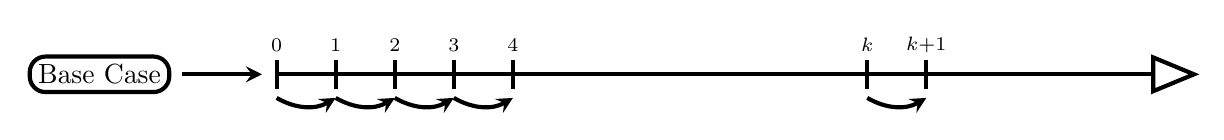
\begin{tikzpicture}[scale=0.75]
            \node[draw,rounded corners=.2cm,inner sep=3pt,line width=1.5pt] (basecase) at (-3, 0) {Base Case};
            \coordinate (0) at (0,0);
            \coordinate (1) at (1,0);
            \coordinate (2) at (2,0);
            \coordinate (3) at (3,0);
            \coordinate (4) at (4,0);
            \coordinate (k) at (10,0);
            \coordinate (k+1) at (11,0);
            \node (n)[isosceles triangle,draw,line width=1.5pt] at (15,0) {};
            
            \draw [line width=1.5pt] (0) -- (n);
            \foreach \lab in {0,1,2,3,4,k,k+1}
                \draw [line width=1.5pt] ($(\lab) + (0,0.25)$) -- ($(\lab) + (0,-0.25)$);
            \foreach \lab in {0,1,2,3,4,k,k+1}
                \node (text\lab) at ($(\lab) + (0,0.5)$) {$\scriptstyle\lab$};

            \draw [->,>=stealth,line width=1.5pt] ($(basecase) + (1.4,0)$) to ($(0) + (-0.25,0)$);

            \draw [->,>=stealth,line width=1.5pt,bend right] ($(0) + (0, -0.4)$) to ($(1) + (0, -0.4)$);
            \draw [->,>=stealth,line width=1.5pt,bend right] ($(1) + (0, -0.4)$) to ($(2) + (0, -0.4)$);
            \draw [->,>=stealth,line width=1.5pt,bend right] ($(2) + (0, -0.4)$) to ($(3) + (0, -0.4)$);
            \draw [->,>=stealth,line width=1.5pt,bend right] ($(3) + (0, -0.4)$) to ($(4) + (0, -0.4)$);
            
            \draw [->,>=stealth,line width=1.5pt,bend right] ($(k) + (0, -0.4)$) to ($(k+1) + (0, -0.4)$);
        \end{tikzpicture}
        \label{fig1}
    \end{figure}

More concretely, an inductive proof has three components: The base cases, the inductive hypothesis, and the inductive step.

\begin{enumerate}
    \item \textbf{Bases Cases} - We first verify that the statement holds for the minimal cases (the ones that start the chain of implications).
    \item \textbf{Inductive Hypothesis} - We want to show that \emph{if} some earlier cases satisfy the statement, \emph{then} so do the subsequent cases. The inductive hypothesis is the \emph{if} part of this if-then statement. We do this by assuming that the statement holds for some or all earlier cases.
    \item \textbf{Inductive Step} - We use the inductive hypothesis to prove that the subsequent cases also hold. This is the \emph{then} part of the if-then statement.
\end{enumerate}

As an example, we can then use this proof technique to prove the following proposition.

\begin{proposition}\label{prop1}
    For all \(n \in \ZZ\), we have that:
    \[\sum_{i=0}^n i = \frac{n(n+1)}{2}\]
\end{proposition}
\begin{proof}
    We prove this by induction over \(n \in \ZZ\).
    
    \textbf{Base Case}: We verify that the proposition holds for \(n=0\). We have that \(\sum_{i=0}^0 i = 0\) which is equal to \(\frac{0 \cdot (0 + 1)}{2} = 0\). And thus, the proposition holds for \(n=0\).

    \textbf{Inductive Hypothesis}: Assume that for some arbitrary \(k \geq 0\) the proposition holds, i.e.,
    \[\sum_{i=0}^k i = \frac{k(k+1)}{2}\]

    \textbf{Inductive Step}: Consider the sum of integers from \(0\) to \(k+1\), we want to show the following.
    \[\sum_{i=0}^{k+1} i = \frac{(k+1)(k+2)}{2}\]
    We do this in the following way using the inductive hypothesis.
    \begin{align*}
        \sum_{i=0}^{k+1} i &= (k+1) + \sum_{i = 0}^{k} i \\
        &= (k+1) + \frac{k(k+1)}{2}\ \ \ \ \text{(by inductive hypothesis)} \\
        &= \frac{2(k+1) + k(k+1)}{2} \\
        &= \frac{k^2 + 3k + 2}{2} \\ 
        &= \frac{(k+1)(k+2)}{2} \\ 
    \end{align*}
    And thus, by induction, the proposition holds for all \(n \in \ZZ\).
\end{proof}

\begin{remark}
    There are many ways to write an inductive hypothesis. For example, we could have said something like ``Fix a \(k \geq 0\), and suppose that the proposition holds." Or we could continue using \(n\) instead of introducing a new variable \(k\). However, be careful. A common mistake is to beg the question/assume the conclusion. That is, if we were to assume that the entire proposition is true. As an incorrect example, I could have said, ``Suppose that for all \(k \geq 0\), the proposition is true." This, however, is incorrect. The goal is to prove the proposition, and so assuming that it is already true defeats the purpose. Instead, we want to fix a \(k\) that is at least as large as our largest base case (in this case \(n=0\)) and assume that the proposition holds for this specific fixed \(k\). This may seem pedantic, but it is important to have the correct wording as otherwise, it can lead to proving incorrect statements.
\end{remark}

The above proof by induction is an example of \emph{weak induction}, the most basic form of induction. In short, weak induction is when we only have a single base case, and the inductive hypothesis only assumes the statement is true for some fixed \(k\).

Now that we have looked at an example, we can formalize this model of induction. We state the Principle or Law of Weak Induction (also called the axiom of induction), which is why induction works.

\begin{definition}[Law of Weak Induction]
    Let \(P(n)\) be a statement regarding a natural number, \(n \in \ZZ\). If 
    \begin{enumerate}
        \item \(P(0)\) is true and
        \item \(\forall k \geq 0 : P(k) \ra P(k+1)\) is true
    \end{enumerate}
    then \(\forall n \geq 0 : P(n)\) is true.
\end{definition}

This law is not proven and is instead typically given as an axiom. It is for this reason we give it as a definition. Additionally, this is also the reason why you should always say something along the lines of, ``And thus, by induction, the proposition holds for all \(n \in \ZZ\)" at the end of your inductive proof. 

\begin{remark}
    It is often the case that some statements are not true for small values of \(n < c\) bellow some fixed constant \(c \in \ZZ\) but are true for all \(n \geq c\). We can still use the Law of Weak Induction in these cases. If we seek to prove that \(\forall n \geq c : P(n)\), then we could instead consider the statement \(Q(n) : P(n + c)\). Then proving that \(\forall n \geq 0: Q(n)\) is equivalent to \(\forall n \geq c : P(n)\).
\end{remark}

\phantom{spacer. I could also use vspace if i wanted to}

Finally, we dissect the law of weak induction to understand how our proof of \cref{prop1} fits into this framework. We first prove the base case, this is the \(P(0)\) part. Then we fixed a \(k\) and showed that \(P(k) \ra P(k+1)\). This is both the inductive hypothesis (assuming \(P(k)\) for some fixed \(k\)) and the inductive step (proving the implication itself). Note that we never wrote the \(\forall k \geq 0\) part in the proof. This is because it is implicit. That is, the inductive hypothesis and inductive step we gave works for any \(k \geq 0\) and so by only considering an arbitrary \(k\) the proof we gave works for all \(k \geq 0\). All in all, this proves the second condition, \(\forall k \geq 0 : P(k) \ra P(k+1)\).

To emphasise this point more, let's say we are trying to prove the following proposition. We can then use use the law of induction in a proof in the following way.

\begin{proposition*}[Template Proposition]
    \(\forall n \geq 0 : P(n)\) is true.
\end{proposition*}
\begin{proof}[Template proof]
    We prove that \(\forall n \geq 0 : P(n)\) is true by induction over \(n \geq 0\).
    
    \textbf{Base Case}: Verify \(P(0)\) is true.

    \textbf{Inductive Hypothesis}: Fix a \(k \geq 0\) and suppose that \(P(k)\) is true.

    \textbf{Inductive Step}: Show that \(P(k) \ra P(k+1)\) is true.

    Then, by the law of (weak) induction, we have proven that \(\forall n \geq 0 : P(n)\).
\end{proof}
 
\subsection{Strong Induction}

So far, we have looked at weak induction. Another form of induction that is widely used is \emph{strong induction}. In short, strong induction is more relaxed. For the inductive hypothesis, we can assume the statement holds for all cases \(m \leq k\), for some fixed \(k\), and not just for \(k\) alone. Before we go further into this technique, we state the Law of Strong Induction.

\begin{definition}[Law of Strong Induction]
    Let \(P(n)\) be a statement regarding a natural number, \(n \in \ZZ\). If
    \begin{enumerate}
        \item \(P(0)\) is true and
        \item \(\forall k \geq 0 : (\forall j \leq k :  P(k)) \ra P(k+1)\) is true
    \end{enumerate}    
    then \(\forall n \geq 0 : P(n)\) is true.
\end{definition}

\begin{remark}
Somewhat surprisingly, strong induction and weak induction are equally as powerful. That is, any proof using strong induction can be converted into a proof using weak induction and vice versa. This is evident by constructing the statement \(Q(n): \forall 0 \leq k \leq n : P(k)\), then using weak induction to prove \(\forall n \geq 0 : Q(n)\) is equivalent to using strong induction to prove \(\forall n \geq 0 : P(n)\). However, in practice, it may be easier to use one over the other.
\end{remark}

As we did for weak induction, we can look at a template proof using strong induction.

\begin{proposition*}[Template Proposition]
    \(\forall n \geq 0 : P(n)\) is true.
\end{proposition*}
\begin{proof}[Template proof]
    We prove that \(\forall n \geq 0 : P(n)\) is true by induction over \(n \geq 0\).
    
    \textbf{Base Case}: Verify \(P(0)\) is true.

    \textbf{Inductive Hypothesis}: Fix a \(k \geq 0\) and suppose that \(\forall j \leq k: P(k)\) is true.

    \textbf{Inductive Step}: Show that \(\left(\forall j \leq k: P(k)\right) \ra P(k+1)\) is true.

    Then, by the law of (strong) induction, we have proven that \(\forall n \geq 0 : P(n)\).
\end{proof}

Notice the only difference between strong and weak induction is the inductive hypothesis. Pictorially, this makes the chain of implications look like the following.

\begin{figure}[ht]
        \centering
        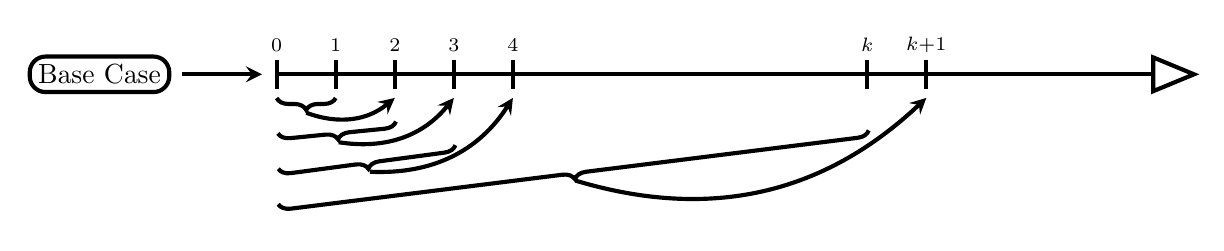
\begin{tikzpicture}[scale=0.75]
            \node[draw,rounded corners=.2cm,inner sep=3pt,line width=1.5pt] (basecase) at (-3, 0) {Base Case};
            \coordinate (0) at (0,0);
            \coordinate (1) at (1,0);
            \coordinate (2) at (2,0);
            \coordinate (3) at (3,0);
            \coordinate (4) at (4,0);
            \coordinate (k) at (10,0);
            \coordinate (k+1) at (11,0);
            \node (n)[isosceles triangle,draw,line width=1.5pt] at (15,0) {};
            
            \draw [line width=1.5pt] (0) -- (n);
            \foreach \lab in {0,1,2,3,4,k,k+1}
                \draw [line width=1.5pt] ($(\lab) + (0,0.25)$) -- ($(\lab) + (0,-0.25)$);
            \foreach \lab in {0,1,2,3,4,k,k+1}
                \node (text\lab) at ($(\lab) + (0,0.5)$) {$\scriptstyle\lab$};

            \draw [->,>=stealth,line width=1.5pt] ($(basecase) + (1.4,0)$) to ($(0) + (-0.25,0)$);

            \draw[decorate, decoration={brace, amplitude=1ex, raise=1ex},line width=1.5pt] ($(1) + (0, -0.2)$) -- ($(0) + (0, -0.2)$) node[pos=.5, left=2.5ex] {};
            \draw [->,>=stealth,line width=1.5pt,bend right] ($0.5*(0) + 0.5*(1) + (0, -0.65)$) to ($(2) + (0, -0.4)$);

            \draw[decorate, decoration={brace, amplitude=1ex, raise=1ex},line width=1.5pt] ($(2) + (0, -0.6)$) -- ($(0) + (0, -0.8)$) node[pos=.5, left=2.5ex] {};
            \draw [->,>=stealth,line width=1.5pt,bend right] ($0.5*(0) + 0.5*(2) + (0.05, -1.15)$) to ($(3) + (0, -0.4)$);

            \draw[decorate, decoration={brace, amplitude=1ex, raise=1ex},line width=1.5pt] ($(3) + (0, -1)$) -- ($(0) + (0, -1.4)$) node[pos=.5, left=2.5ex] {};
            \draw [->,>=stealth,line width=1.5pt,bend right] ($0.5*(0) + 0.5*(3) + (0.08, -1.65)$) to ($(4) + (0, -0.4)$);

            \draw[decorate, decoration={brace, amplitude=1ex, raise=1ex},line width=1.5pt] ($(k) + (0, -0.75)$) -- ($(0) + (0, -2)$) node[pos=.5, left=2.5ex] {};
            \draw [->,>=stealth,line width=1.5pt,bend right] ($0.5*(0) + 0.5*(k) + (0.06, -1.8)$) to ($(k+1) + (0, -0.4)$);
        \end{tikzpicture}
        \label{fig2}
    \end{figure}

As a side note, in future classes, and maybe in this one too, we will see what are called loop invariant proofs, which use weak induction under the hood. That is, they assume only that the loop invariant is true at the start of the loop and then prove that it is true at the end of the loop (or at the start of the next iteration, depending on how you phrase it). In comparison, many proofs for recursive algorithms use strong induction. That is, they assume that the algorithm works for subproblems of smaller sizes.
% See \cref{section_rec_alg_correctness} for more info.

We can then give some examples of using strong induction.

\begin{proposition}
    Let \(F_n\) for \(n \geq 0\) denote the \(n\)th Fibonacci number, which is defined as \(F_0 = 0, F_1 = 1, F_n = F_{n-1} + F_{n-2}\) for \(n \geq 2\). And let \(L_n\) for \(n \geq 0\) denote the \(n\)th Lucas number, which is defined as \(L_0 = 2, L_1 = 1, L_n = L_{n-1} + L_{n-2}\) for \(n \geq 2\). We have that for all \(n \geq 1\),
    \[L_n = F_{n-1} + F_{n+1}\]
\end{proposition}

For reference, we write the first few numbers for both sequences:
\[\begin{array}{c|c|c|c|c|c|c|c|c}
    n   & 0 & 1 & 2 & 3 & 4 & 5 & 6 & 7 \\
    \hline \hline
    F_n & 0 & 1 & 1 & 2 & 3 & 5 & 8 & 13 \\
    \hline
    L_n & 2 & 1 & 3 & 4 & 7 & 11 & 18 & 29 \\
\end{array}\]

\begin{proof}
    We prove this by strong induction over \(n \geq 1\).
    
    \textbf{Base Case}: We verify that the proposition holds for \(n=1\) and \(n=2\). First, we can verify that \(L_1 = 1\) and \(F_0 + F_2 = 0 + 1 = 1\). Next, we can verify that \(L_2 = 3\) and \(F_1 + F_3 = 1 + 2 = 3\). And thus, the proposition holds for \(n=1\) and \(n=2\).

    \textbf{Inductive Hypothesis}: Assume that for some arbitrary \(k \geq 2\) the proposition holds for \(k\) and \(k-1\):
    \[L_k = F_{k-1} + F_{k+1}\]
    \[L_{k-1} = F_{k-2} + F_{k}\]

    \textbf{Inductive Step}: Consider the \((k+1)\)th Lucas number, which we want to show is \(L_{k+1} = F_{k} + F_{k+2}\). We do this in the following way.
    % \begin{align*}
    %     L_{k+1} &= L_{k} + L_{k-1}\ \ \ \ \ \ \ \ \ \ \ \ \ \ \ \ \ \ \ \ \ \ \ \ \text{(by definition of the Lucas numbers)} \\
    %     &= F_{k-1} + F_{k+1} + F_{k-2} + F_{k}\ \ \ \ \text{(by inductive hypothesis)} \\
    %     &= F_{k} + F_{k+2}\ \ \ \ \ \ \ \ \ \ \ \ \ \ \ \ \ \ \ \ \ \ \ \ \,\text{(by definition of the Fibonacci numbers)}
    % \end{align*}
    \[\begin{array}{rll}
        L_{k+1} \!\!\!\! &= L_{k} + L_{k-1} & \text{(by definition of the Lucas numbers)} \\
        &= F_{k-1} + F_{k+1} + F_{k-2} + F_{k} & \text{(by inductive hypothesis)} \\
        &= F_{k} + F_{k+2} & \text{(by definition of the Fibonacci numbers)}
    \end{array}\]
    And thus, by induction, the proposition holds for all \(n \geq 1\).
\end{proof}

\begin{remark}
    In this proof, we used two base cases and assumed the proposition held for both \(n=k\) and \(n=k-1\), but why is this? You will notice that in the inductive step, we applied the inductive hypothesis to both \(L_k\) and \(L_{k-1}\). If we only assumed it held for \(n=k\), then we would be left with \(L_{k+1} = F_{k-1} + F_{k+1} + L_{k-1}\), which wouldn't help us prove the proposition for \(n=k+1\). Next, for the base cases, if we were only to have one base case, for \(n=1\), then the inductive hypothesis would have to consider some fixed \(k \geq 1\). For the smallest value of \(k=1\), this would have us assume that \(L_0 = F_{-1} + F_{1}\), which doesn't make sense as negative Fibonacci numbers haven't been defined in this proposition. As a general rule of thumb, the number of required base cases equals the number of assumptions you make in the inductive hypothesis (this isn't always true, but it often a good rule of thumb to start with).
\end{remark}

\phantom{abc}

Next, we will look at the tournament ranking problem 
\footnote{Quick integrity check. This problem is often given as homework; if you use this solution at any step while doing your homework for a future or current class, you should always cite your sources.}.
So far, all the proofs in this document have only concerned numerical equalities. However, this is a computer science class, and so we want to prove things that are more relevant to algorithms. The tournament ranking is a nice introduction to this.

\begin{proposition}[The Tournament Ranking Problem]
    Consider a tennis tournament of \(n \geq 1\) players, denoted by \(\left\{P_1, P_2, \dotsc, P_n\right\}\). For each pair of players, say \(\{P_i, P_j\}\), they play a match where one player wins (there are no ties). We say \(P_i \prec P_j\) if player \(P_j\) beats \(P_i\) in their match. Then for any outcome of the \(\binom{n}{2}\) matches, there is always an ordering of the players:
    \[P_{i_1} \prec P_{i_2} \prec \cdots \prec P_{i_n}\]
    Here, \(i_1, i_2, \dotsc, i_n\) denotes a permutation of \(1, 2, \dotsc, n\). Note, an ordering is \emph{not} transitive, that is, for players \(\{P_1, P_2, P_3\}\), \(P_1 \prec P_2 \prec P_3\) does \emph{not} imply \(P_1 \prec P_3\), rather only that \(P_1 \prec P_2\) and \(P_2 \prec P_3\).
\end{proposition}

\phantom{ignore me}

Before we prove this, it is useful to give the idea of the proof. That is, for our tournament of \(n\) players, which, for notation we will call \(\text{PLAYERS} = \left\{P_1, P_2, \dotsc, P_n\right\}\), we fix player \(P_1\) and consider all the players that lost to player \(P_1\) and all the players that beat \(P_1\). That is, we consider all the players that can go where the \(??\)s are:
\[?? \prec P_1 \prec ??\]
Furthermore, the number of players that can go where the \(??\)s are is strictly less than \(n\) as they can't include \(P_1\). This defines a recursive structure of the problem. Namely, if we can find an ordering of these subsets of players and put them where the question marks are, we would get an ordering for all \(n\) players.

To make the proof easier, we will consider the base case to be when there are no players in the tournament. Even though we only need to prove this proposition for \(n \geq 1\), we will find it to be much easier to prove it for \(n \geq 0\). This may seem weird at first, but everything works out as far as the induction step is concerned.

\begin{proof}
    We prove this by strong induction over the number of players in the tournament, \(n \geq 0\).
    
    \textbf{Base Case}: We verify that there exists an ordering for no player, \(\emptyset\). The ordering is nothing.

    \textbf{Inductive Hypothesis}: Assume that for some \(k \geq 0\), any tournament of \(0 \leq m \leq k\) players has an ordering of the players.

    \textbf{Inductive Step}: Consider a tournament of \(k+1\) players and let \(\text{PLAYERS} = \left\{P_1, P_2, \dotsc, P_k, P_{k+1}\right\}\) be the set of the players. We then fix \(P_1\) and consider the set of players that lost to \(P_1\), which we will call \(L\), and the set of players that beat \(P_1\), which we will call \(W\). These sets can be defined by 
    \[L = \{P \in \text{PLAYERS}\ |\ P \prec P_1\}\]
    \[W = \{P \in \text{PLAYERS}\ |\ P_1 \prec P\}\]

    Because \(P_1 \notin L\) and \(P_1 \notin W\) we have that \(s = |L| \leq k\) and \(t = |W| \leq k\). Furthermore, because no player can both lose and win to \(P_1\) and every player had a match with \(P_1\), they are disjoint, and their union is all players minus \(P_1\). We can then use the induction hypothesis to get an ordering of the players in \(L\) and \(W\) (that is, we consider ``sub-tournaments" of only the matches between the players in \(L\) and \(W\)). Let the orderings for \(L\) and \(W\) be given by the following, respectively:
    \[P_{\ell_1} \prec P_{\ell_2} \prec \cdots \prec P_{\ell_s}\]
    \[P_{w_1} \prec P_{w_2} \prec \cdots \prec P_{w_s}\]
    Finally, we can construct the final ordering as follows. Note, if either \(L\) or \(W\) are the empty set, then we ignore their orderings and let \(P_1\) be at one or both of the ends of the ordering.
    \[P_{\ell_1} \prec \cdots \prec P_{\ell_s} \prec P_1 \prec P_{w_1} \prec \cdots \prec P_{w_s}\]
    All that is left to check is that \(P_{\ell_s} \prec P_1\) and \(P_1 \prec P_{w_1}\). These follow from the fact that \(P_{\ell_s} \in L\) and thus lost to \(P_1\) and that \(P_{w_1} \in W\) and thus beat \(P_1\).

    Thus, by induction, there is always an ordering for any tournament of \(n \geq 1\) players.
\end{proof}

\begin{remark}
    In many ways, the inductive step can be seen as proving the correctness of a recursive algorithm for finding an ordering. This algorithm is a divide-and-conquer style strategy that can be roughly written in the following way: We first divide the problem into the losing and winning sets, then we find an ordering for them recursively, and finally, we combine them together to get an ordering for the whole set. Then, proving the proposition is equivalent to proving the correctness of this algorithm (which is written in pseudo-code below). Note we store this ordering in a list data structure that supports list concatenation with the \(+\) operator.
    \begin{algorithm}[Tournament Ranking Algorithm] \phantom{}\label{alg_tourn_ranking}
    
    \begin{center}
    \begin{minipage}{.5\linewidth}
    \begin{algorithmic}[1]
        \Procedure{\textsc{TournamentRanking}}{\text{PLAYERS}}
            \If{\(\text{PLAYERS} = \emptyset\)} 
                \Return \([\;]\)
            \Else
                \State fix \(P_1 \in \text{PLAYERS}\)
                \State \(L \leftarrow \{P \in \text{PLAYERS}\ |\ P \prec P_1\}\)
                \State \(W \leftarrow \{P \in \text{PLAYERS}\ |\ P_1 \prec P\}\)

                \State \(L_{\text{ord}} \leftarrow \textsc{TournamentRanking}(L)\)
                \State \(W_{\text{ord}} \leftarrow \textsc{TournamentRanking}(W)\)
                
                \State \textbf{return} \(L_{\text{ord}} + [P_1] + W_{\text{ord}}\)
            \EndIf 
        \EndProcedure
    \end{algorithmic}
    \end{minipage}
    \end{center}
    \end{algorithm}
\end{remark}

\subsection{Problems/Exercises}

\begin{problem}
    Prove the following:
    Let \(n \in \ZZZ\), then for two sequences of positive numbers, \((a_i)_{i \in [n]}\) and \((b_i)_{i \in [n]}\) we have that
    \[\min_{i \in [n]} \left(\frac{a_i}{b_i}\right) \leq \frac{\sum_{i = 1}^n a_i}{\sum_{i = 1}^n b_i} \leq \max_{i \in [n]} \left(\frac{a_i}{b_i}\right)\]

    [Hint: First prove the \(n=2\) case, then break up your inductive case into two cases that allow you to use the result of the \(n=2\) case directly. However, your base case should still be when \(n=1\).]
\end{problem}

\begin{problem}
    Prove the following: Let \(F_n\) for \(n \geq 0\) denote the \(n\)th Fibonacci number. Fix an \(n \in \ZZ\), then we have the following
    \[\sum_{i = 0}^n F_n = F_{n+2} - 1\]
\end{problem}

% \section{Proving the Correctness of Recursive Algorithms}\label{section_rec_alg_correctness}

% In this section we look more closely at applying the proof by induction technique to recursive algorithms. As we saw with \cref{alg_tourn_ranking}, a strong induction proof often can been seen as proving the correctness of an algorithm. This is primarily because our proof gave a construction of a ranking. Then, each step in the proof mirrored a step in an algorithm. Moreover, when we used the inductive hypothesis, we assumed that such a construction exist on a smaller tournament sizes. In algorithm terms, we assumed that our algorithm would work for smaller input sizes.

% We can then dissect the parts in a recursive algorithm. Most of the recursive algorithm that we will look at fit the category of a divide-and-conquer algorithm. These have three parts.
% \begin{enumerate}
%     \item \textbf{Divide:} Divide the input into sub-problems of strictly smaller size.
%     \item \textbf{Conquer:} Recursively call the algorithm on these sub-problems.
%     \item \textbf{Combine:} Combine the results of the sub-problems to get a solution for the whole problem.
% \end{enumerate}
% When the problem can't be divided into smaller problems we would have a base case that does simple calculations, usually on instances with constant size. 

% We can then see how this framework mirrors the proof by induction paradigm, and in particular that of strong induction. That is, the correctness of the algorithm depends on the correctness of the base case and the correctness an of the algorithm on arbitrary sized input if it is correct for smaller inputs.

% Consider the following sorting algorithm. We will prove the correctness using proof by induction. Here, by correct, we mean that it correctly sorts a list of numbers.

% \begin{algorithm}[Merge Sort Like Algorithm] To make our life easier, we will assume the input list, \(A[1..n]\), always has a length being a power of 2. \label{alg_merge_sort_like}
    
%     \begin{center}
%     \begin{minipage}{.5\linewidth}
%     \begin{algorithmic}[1]
%         \Procedure{\textsc{Sort}}{$A[1..n]$}
%             \If{\(n > 1\)} 
%                 \State \textsc{Sort}\((A[1..n/2])\)
%                 \State \textsc{Sort}\((A[n/2+1..n])\)
%                 \State \textsc{Merge}\((A[1..n])\)
%             \EndIf 
%         \EndProcedure
%         \State
%         \Procedure{\textsc{Merge}}{$A[1..n]$}
%             \If{\(n = 2\)} 
%                 \If{\(A[1] > A[2]\)}
%                     \State \textsc{Swap}(\(A[1],A[2]\))
%                 \EndIf
%             \Else
%                 \For{\(i\) in \([1..n/4]\)}
%                     \State \textsc{Swap}(\(A[i+n/4],A[i + n/2]\))
%                 \EndFor
%                 \State \textsc{Merge}\((A[1..n/2])\)
%                 \State \textsc{Merge}\((A[n/2+1..n])\)
%                 \State \textsc{Merge}\((A[n/4+1..2n/4])\)
%             \EndIf 
%         \EndProcedure
%     \end{algorithmic}
%     \end{minipage}
%     \end{center}
% \end{algorithm}

% \begin{claim}[Correctness of \cref{alg_merge_sort_like}]
%     \cref{alg_merge_sort_like} correctly sorts a list of numbers.
% \end{claim}

% \begin{proof}
%     TODO
% \end{proof}

\section{Additional Reading}

For a more in-depth resource, Richard Hammacks's \emph{Book of Proof} (Chapter 10) is a great resource. It can be found here: \url{https://www.people.vcu.edu/~rhammack/BookOfProof/}.

Additionally, one of my past TAs, Michael Levet, has an excellent resource on mathematics in computer science, the first chapter of which is on proof by induction: \url{https://michaellevet.github.io/Algorithms_Notes.pdf}

Inspiration for earlier drafts of these notes came, in part, from these two sources.

\end{document}
